
%%% Local Variables:
%%% LaTeX-command: "pdflatex --shell-escape"
%%% End:

\documentclass[11pt]{article}
\usepackage[utf8]{inputenc}
\usepackage[T1]{fontenc}
\usepackage{grffile}
\usepackage{longtable}
\usepackage{wrapfig}
\usepackage{rotating}
\usepackage[normalem]{ulem}
\usepackage{amsmath}
\usepackage{textcomp}
\usepackage{amssymb}
\usepackage{capt-of}
\usepackage{hyperref}
\hypersetup{colorlinks=true, linkcolor=magenta}
\setlength{\parindent}{0in}
\usepackage[margin=0.8in]{geometry}
\usepackage[english]{babel}
\usepackage{mathtools}
\usepackage{palatino}
\usepackage{fancyhdr}
\usepackage{sectsty}
\usepackage{engord}
\usepackage{parskip}
\usepackage{minted}
\usepackage{cite}
\usepackage{graphicx}
\usepackage{subcaption}
\usepackage{setspace}
\usepackage{minted}
\usepackage[compact]{titlesec}
\usepackage{placeins}
\usepackage{color}
\usepackage{amsmath}
\usepackage{bm}
\usepackage{todonotes}
\usepackage{pdfpages}
\titlespacing*{\subsection}
{0pt}{5.5ex plus 1ex minus .2ex}{2.3ex plus .2ex}
\titlespacing*{\section}
{0pt}{5.5ex plus 1ex minus .2ex}{1ex}

\author{Luis Antonio Ortega Andrés \\\medskip Juan Ignacio Álvarez Trejos}
\date{\today}
\title{Auto-encoding Variational Bayes\\\medskip
\large Applied Bayesian Methods}

\begin{document}

\maketitle

The main objective of this assignment is to develop a variational autoencoder using the working principles of variational inference, and, use this method for doing approximate inference in the MNIST dataset. The probabilistic model considered is a generative model of the form:

\begin{figure}[h]
  \centering
  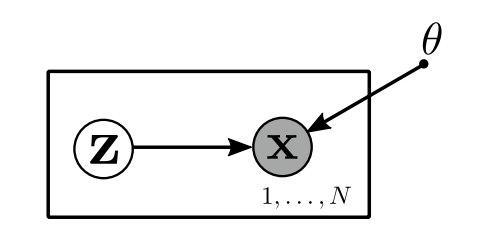
\includegraphics[scale = 0.5]{imgs/model.jpg}
 \end{figure}

 \textbf{Task 1.} \emph{Complete the missing parts of the code to allow for training a VAE on the MNIST dataset.}

 We are briefly reviewing the implemented steps for each of the four functions designed to this task. Let us begin with \texttt{sample\_latent\_variables\_posterior}, the main aim of this function is to generate an unique sample from \( Q(z \mid x) \) for each \( x \) in the given batch. To this end, the mean and variance of each factor \( Q \) is given as input for the function. These values can be retieved form the first and last half over the last axis. In order to return the desired samples we are using the decomposition property of the Gaussian distribution, that is
 \[
   \mathcal{N}(\mu, \sigma^{2}) = \mu + \sigma \mathcal{N}(0, 1).
 \]
 The resulting code is
 \begin{minted}{python}
   mean, log_std = encoder_output[:, :D], encoder_output[:, D:]
   z = npr.randn(*mean.shape)
   return mean + z * np.exp(log_std)
 \end{minted}

 The \texttt{bernoulli\_log\_prob} function aims to return the log-likelihood of the actual data given the computed logits using the output of the neural netork, that is, to compute
 \[
   \begin{aligned}
     \log P(\bm{x} \mid \bm{z}) &= \sum_{x \in \bm{x}}\log\Big(p(x)^{x} + (1-p(x))^{(1-x)}\Big)\\
      &= \sum_{x \in \bm{x}}\log\Big( x\ p(x) + (1-x)\ (1-p(x))\Big).
     \end{aligned}
  \]
  To this end, it is needed to compute the probabilities fro the given logits using the sigmoid function:
  \begin{minted}{python}
    probs = sigmoid(logits)
    log_prob = np.log(targets * probs + (1 - targets) * (1 - probs))
    return np.sum(log_prob, axis=-1)
  \end{minted}
  On the other hand, function \texttt{compute\_KL} is used to compute the Kullback-Leibler divergence between the variational distribution \( Q(\bm{z} \mid \bm{x}) \)  and the prior distirbution \( \mathcal{N}(0, I)\). Given that both distributions are Gaussian, their KL divergence has a closed form which is in turn simplified given the form of the prior. More precisely,
  \[
    \mathcal{KL}\Big( \mathcal{N}\big((\mu_{1}, \dots, \mu_{k})^{T}, \text{diag}(\sigma^{2}_{1}, \dots, \sigma^{2}_{k}) \big) \mid \mathcal{N}(\bm{0}, \bm{I}) \Big) = \frac{1}{2}\sum_{i=1}^{k}\left( \sigma_{i}^{2} + \mu_{i}^{2} - 1 - \log\sigma_{i}^{2} \right).
  \]
  This value can be easily computed given \texttt{mean} and \texttt{log\_stds} from the neural network output as

\begin{minted}{python}
  KL = 0.5 * (np.exp(2 * log_std) + mean ** 2 - 1 - 2 * log_std)
  return np.sum(KL, axis = -1)
\end{minted}

Lastly, \texttt{vae\_lower\_bound} is used to compute a noisy estimate of the lower bound by using a single Monte Carlo sample. That is, to approximate the expectation in the objective function with a single observation of the variable. The steps are the following:
\begin{enumerate}
  \item Compute the encoder output using \texttt{neural\_net\_predict}:
        \begin{minted}{python}
  output = neural_net_predict(params=rec_params, inputs=data)
        \end{minted}
  \item Sample the latent variables associated to the batch in data:
        \begin{minted}{python}
  latents = sample_latent_variables_from_posterior(output)
        \end{minted}
  \item Reconstruct the image and to compute the log likelihood of the actual data:
        \begin{minted}{python}
  x_samples = neural_net_predict(gen_params, latents)
  log_prob = bernoulli_log_prob(data, x_samples)
        \end{minted}
  \item Compute the KL divergence between \( Q(\bm{z} \mid \bm{x}) \)  and the prior:
        \begin{minted}{python}
  KL = compute_KL(output)
        \end{minted}
  \item Estimate the lower bound by substracting the KL to the data dependent term
        \begin{minted}{python}
  return np.mean(log_prob - KL, axis=-1)
        \end{minted}
\end{enumerate}

\textbf{Task 2.} \emph{Complete the initialization of the ADAM parameters and write the ADAM updates
in the main training loop of the code provided in \texttt{vae.py}}.

Using the provided description of the algorithm, the parameter updates can be computed as the following:
\begin{minted}{python}
  m = beta1 * m + (1 - beta1) * grad
  v = beta2 * v + (1 - beta2) * grad ** 2
  m_unbiased = m / (1 - beta1 ** t)
  v_unbiased = v / (1 - beta2 ** t)

  flattened_current_params += (
        alpha * m_unbiased / (np.sqrt(v_unbiased) + epsilon)
  )
\end{minted}
With initial values given by
\begin{minted}{python}
  alpha = 0.001
  beta1 = 0.9
  beta2 = 0.999
  epsilon = 1e-8
  m = np.zeros_like(flattened_current_params)
  v = np.zeros_like(flattened_current_params)
\end{minted}

\end{document}
